\section[C]{The Linear Expenditure System}\label{LES}

\setlength{\parskip}{0.2in}

The linear expenditure system (\textsc{les} or \textit{Stone-Geary})
utility function was invented by Roy Geary and first estimated by
Richard Stone.  An early analysis by \cite{frisch} calibrated the
functional form using a parameter named the `money flexibility'.
Subsequently, \cite{sato} and \cite{powell} pointed out the
correspondence between Frisch's money flexibility and the elasticity
of substitution among commodities.  Here we employ Powell's insight to
calibrate the linear expenditure demand system to benchmark data
consisting of expenditure shares, income elasticities of demand and
the share-weighted compensated elasticity of demand.

Let $x_i$ denote aggregate demand for good $i$.  In the \textsc{les}
demand system, $x_i$ is the sum of subsistence demand ($s_i$) and
discretionary demand ($d_i$).  Subsistence demand remains fixed on a
per-capita basis while discretionary demand depends on commodity
prices and income.

Given homogeneity of prices we may assume that the benchmark
expenditure and prices of all goods equal unity, and the benchmark
demand for commodity $i$ equals $\theta_i$, the benchmark
value share of commodity $i$ in final demand.  Demand for $i$
resulting from \textsc{les} utility maximization can be written:
\begin{equation}
\label{lesdemand}
x_i  =  s_i + \bar d_i \frac{1 - \sum_j p_j s_j}{\beta p_i} 
= s_i + \bar d_i \frac{c(p)}{p_i} u 
\end{equation}
where \begin{description}
\item[$M$] indicates income (equal to unity at the benchmark point),  
\item[$p_i$] is the price of good $i$ (equal to unity at the benchmark
point), 
\item[$\beta$] is the benchmark value share of
discretionary demand $\left( = \sum_i \bar d_i \right)$, 
\item[$\alpha_i$] is the value share of
good $i$ in discretionary demand $\left( = \frac{\bar d_i}{\beta}
\right)$
\item[$c(p)$] is the price index of discretionary demand $\left(= \prod_i
p^{\alpha_i}_i \right)$, and 
\item[$u$] is an indirect
utility index for discretionary demand\footnote{The money-metric
utility index for aggregate utility is $U = 1 + \beta (u - 1)$} 
$\left( = \frac{M - \sum_j p_j s_j}{\beta c(p)} \right)$
\end{description}

Utility maximization provides a demand function $x_i(p,M)$.  In
the \textsc{gtap} setting, inputs to the demand system calibration are:
\begin{itemize}
\item[$\theta_i$]       The expenditure share of good $i$
\item[$\epsilon_i$]     The compensated own-price elasticity of demand:
$$\epsilon_i = \left. \frac{\partial x_i(p,M(U))}{\partial p_i}\right|_{U=\bar
U} \frac{p_i}{x_i}$$
\item[$\eta_i$]         The income elasticity of demand for good $i$
$$\eta_i = \frac{\partial x_i(p,M)}{\partial M} \frac{M}{x_i}.$$
\end{itemize}

Calibration of the \textsc{les} to $\theta_i$, $\epsilon_i$ and
$\eta_i$ involves allocating budget shares across
subsistence and discretionary demand, subject to the constraint:
$$\theta_i = s_i + \bar d_i$$ 
Differentiating (\ref{lesdemand}) with respect to $M$, the income
elasticity of demand is given by:
$$\eta^{\rm \textsc{les}}_i = \frac{1}{\beta} \left( 1 - \frac{s_i}{\theta_i} \right)$$

This expression permits us to calibrate $s_i$ and $\bar d_i$ in terms
of $\theta_i$, $\beta$ and $\eta_i$:
$$s_i = \theta_i (1 - \beta \eta_i)$$
and 
$$\bar d_i = \theta_i - s_i = \beta \eta_i \theta_i.$$
and hence $\alpha_i = \eta_i \theta_i$.

Diagonal terms in the Slutsky matrix of the \textit{compensated}
demand function at the benchmark point can be found by differentiating 
(\ref{lesdemand}), holding $u=1$:
$$\frac{\partial x_i}{\partial p_i} = \bar d_i (\alpha_i - 1),$$
hence
\begin{equation}
\label{epsilondef}
\epsilon^{\rm \textsc{les}}_i = \beta \eta_i ( \alpha_i  - 1) = \beta \eta_i (
\eta_i \theta_i - 1) 
\end{equation}

The discretionary expenditure share, $\beta$, is a free parameter
which can be calibrated to target \textit{average} compensated price
elasticities, i.e.
$$\min_\beta \sum_i \theta_i \left( \epsilon_i - \beta \eta_i \left(
\eta_i \theta_i - 1 \right) \right)^2,$$
hence, if we calibrate $\beta$ from to match average own-price
elasticities, we have:
$$ \beta = \frac{\sum_i \theta_i \epsilon_i}{\sum_i \eta_i
\theta_i (\eta_i \theta_i - 1)}$$

One consequence of this calibration is that when elasticities are
high, subsistence demands may be negative, producing some difficulty
in interpretation.  An alternative approach is to fix $\beta$ at
maximum value for which subsistence demands are
non-negative:
$$\beta = \min_i \frac{1}{\eta_i} = \frac{1}{\eta_{\rm max}},$$
and then replace the Cobb-Douglas utility function over discretionary
demand with a constant-elasticity-of-sustitution (\textsc{ces}) utility function.
The unit cost function is then
$$c^{\rm \textsc{ces}}(p) = \left(\sum_i \eta_i \theta_i p_i^{1-\sigma}
\right)^{1/(1-\sigma)}$$
and the demand function is
$$x_i = s_i + \bar d_i \left( \frac{c^{\rm \textsc{ces}}(p)}{p_i} \right)^\sigma
u.$$ 
Given any value of $\beta$, the elasticity of substitution in 
discretionary demand can then be calibrated to match the average
own-price elasticity:
$$\sigma = \frac{ \sum_i \theta_i \epsilon_i}{\beta \sum_i \eta_i
\theta_i (\eta_i \theta_i - 1)}.$$

%	These figures are from LESModel.xlsm which is included in the 
%	LaTeX/figures directory:

\begin{figure}
\begin{minipage}[b]{.3\linewidth}
\centering
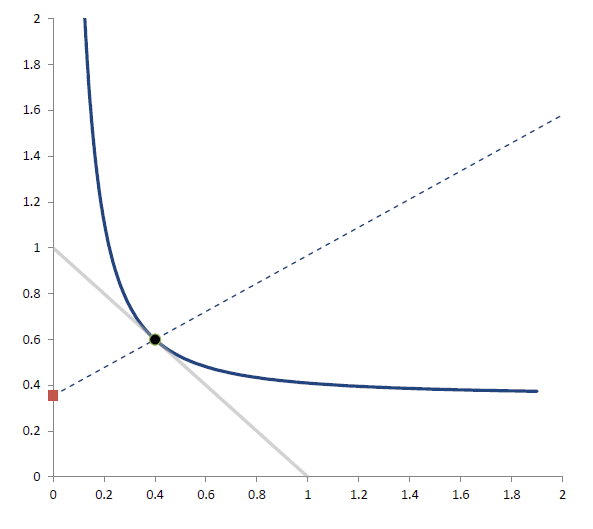
\includegraphics[width=2in]{figures/65.png}
\subcaption{$\beta=0.65$, $\bar \epsilon = -0.28$}
\end{minipage}
\begin{minipage}[b]{.3\linewidth}
\centering
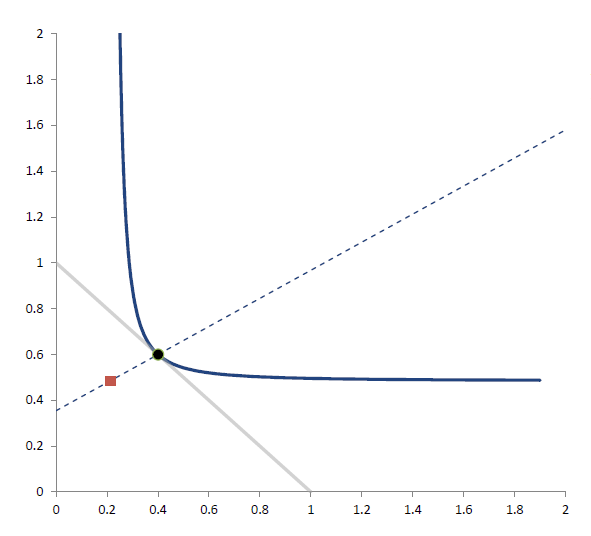
\includegraphics[width=2in]{figures/35.png}
\subcaption{$\beta=0.30$, $\bar \epsilon = -0.14$}
\end{minipage}
\begin{minipage}[b]{.3\linewidth}
\centering
..
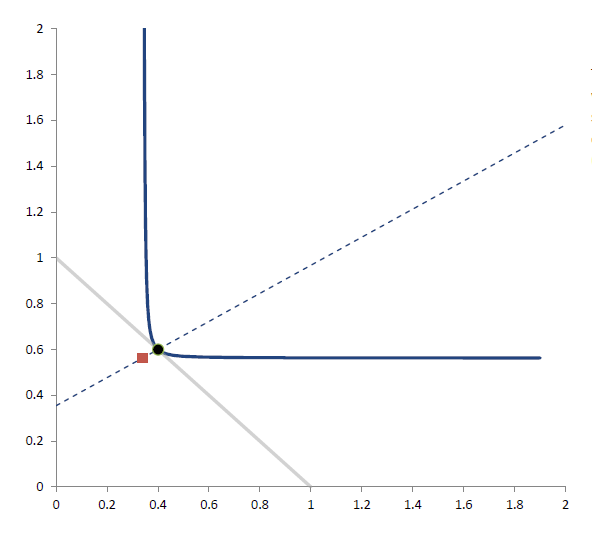
\includegraphics[width=2in]{figures/10.png}
\subcaption{$\beta=0.10$, $\bar \epsilon = -0.05$}
\end{minipage}
\caption{Calibration with Alterative Price Elasticities}
\end{figure}
